\documentclass[11pt,a4paper,dvipdfmx]{article}
%\documentclass[autodetect-engine,dvipdfmx-if-dvi,ja=standard]{bxjsarticle}

\usepackage[utf8]{inputenc}
\usepackage{lmodern}
\usepackage[T1]{fontenc}
\usepackage[noBBpl]{mathpazo}
%\linespread{1.05}
\usepackage{mathtools, amsmath, amssymb, amsthm}
\usepackage{amsfonts}
\usepackage{braket}
%\usepackage{amssymb}
\usepackage{url}
\usepackage{cases}

%% citation
\usepackage[longnamesfirst]{natbib}

%
\theoremstyle{plain}
\newtheorem{thm}{Thm.}[section]
\newtheorem{lem}{Lem.}[section]
\newtheorem{cor}{Cor.}[section]
\newtheorem{prop}{Prop.}[section]
\newtheorem{df}{Def.}[section]
\newtheorem{eg}{e.g.}[section]
\newtheorem{rem}{Rem.}[section]
%

\usepackage{listings}
\lstset{%
language={python},%
basicstyle={\ttfamily\footnotesize},%ソースコードの文字を小さくする
frame={single},
commentstyle={\footnotesize\itshape},%コメントアウトの文字を小さくする
breaklines=true,%行が長くなったときの改行。trueの場合は改行する。
numbers=left,%行番号を左に書く。消す場合はnone。
xrightmargin=3zw,%左の空白の大きさ
xleftmargin=3zw,%右の空白の大きさ
stepnumber=1,%行番号を1から始める場合こうする(たぶん)
numbersep=1zw,%行番号と本文の間隔。
}

%\usepackage[dvipdfmx]{graphicx}
%% color packageとdvipdfmxは相性が悪いらしい
%% https://qiita.com/zr_tex8r/items/442b75b452b11bee8049
\usepackage{graphicx}


\usepackage[left=2cm,right=2cm,top=2cm,bottom=2cm]{geometry} %This changes the margins.
\usepackage{float}
%\author{Kyohei Okumura}
\global\long\def\T#1{#1^{\top}}

\newcommand{\id}{\textnormal{id}}
\newcommand{\R}{\mathbb{R}}
\newcommand{\N}{\mathbb{N}}
\newcommand{\Q}{\mathbb{Q}}
\newcommand{\Z}{\mathbb{Z}}
\newcommand{\C}{\mathbb{C}}
\newcommand{\mF}{\mathcal{F}}
\newcommand{\mG}{\mathcal{G}}
\newcommand{\mA}{\mathcal{A}}
\newcommand{\mB}{\mathcal{B}}
\newcommand{\mC}{\mathcal{C}}
\newcommand{\mD}{\mathcal{D}}
\newcommand{\mL}{\mathcal{L}}
\newcommand{\mM}{\mathcal{M}}
\newcommand{\mO}{\mathcal{O}}
\newcommand{\mP}{\mathcal{P}}
\newcommand{\mS}{\mathcal{S}}
\newcommand{\mT}{\mathcal{T}}
\newcommand{\mV}{\mathcal{V}}
\renewcommand{\Re}{\mathrm{Re}}
\renewcommand{\hat}{\widehat}
\renewcommand{\tilde}{\widetilde}
\renewcommand{\bar}{\overline}
\renewcommand{\epsilon}{\varepsilon}
% \renewcommand{\span}{\mathrm{span}}
\newcommand{\defi}{\stackrel{\Delta}{\Longleftrightarrow}}
\newcommand{\equi}{\Longleftrightarrow}
\newcommand{\s}{\succsim}
\newcommand{\p}{\precsim}
\newcommand{\join}{\vee}
\newcommand{\meet}{\wedge}
\newcommand{\1}{\mbox{1}\hspace{-0.25em}\mbox{l}}

\DeclareMathOperator{\Var}{Var}
\DeclareMathOperator{\Cov}{Cov}
\DeclareMathOperator{\sgn}{sgn}
\DeclareMathOperator{\Card}{Card}
\DeclareMathOperator{\supp}{supp}
\DeclareMathOperator{\Log}{Log}
\DeclareMathOperator{\spn}{span}

\newcommand{\indep}{\mathop{\perp\!\!\!\!\perp}}

\usepackage{color}
\newcommand{\kcomment}[1]{{\textcolor{blue}{#1}}}
\newcommand{\ocomment}[1]{{\textcolor{red}{#1}}}


\begin{document}
\title{SML HW6}
\author{29-176004 奥村 恭平{\footnote{E-mail: kyohei.okumura@gmail.com}
\footnote{東京大学大学院 経済学研究科 M2}
}}
\date{\today}
\maketitle

%%%%%%%%%%%%%%%%%%%%%%%%%%%%%%%%%%%%%%%%%%%%%%%%%%%%%%%%%%%

\section*{宿題1: カーネル密度推定法の実装}
ガウスカーネルに対するカーネル密度推定法を実装した.(言語はpython.)
バンド幅は尤度交差確認により決定($b^* := 0.1$)した.
以下はシミュレーション結果の図.上がオリジナルのサンプルのヒストグラム,下が推定された密度関数.うまく推定できていることがわかる.

\begin{figure}[H]
  \centering
    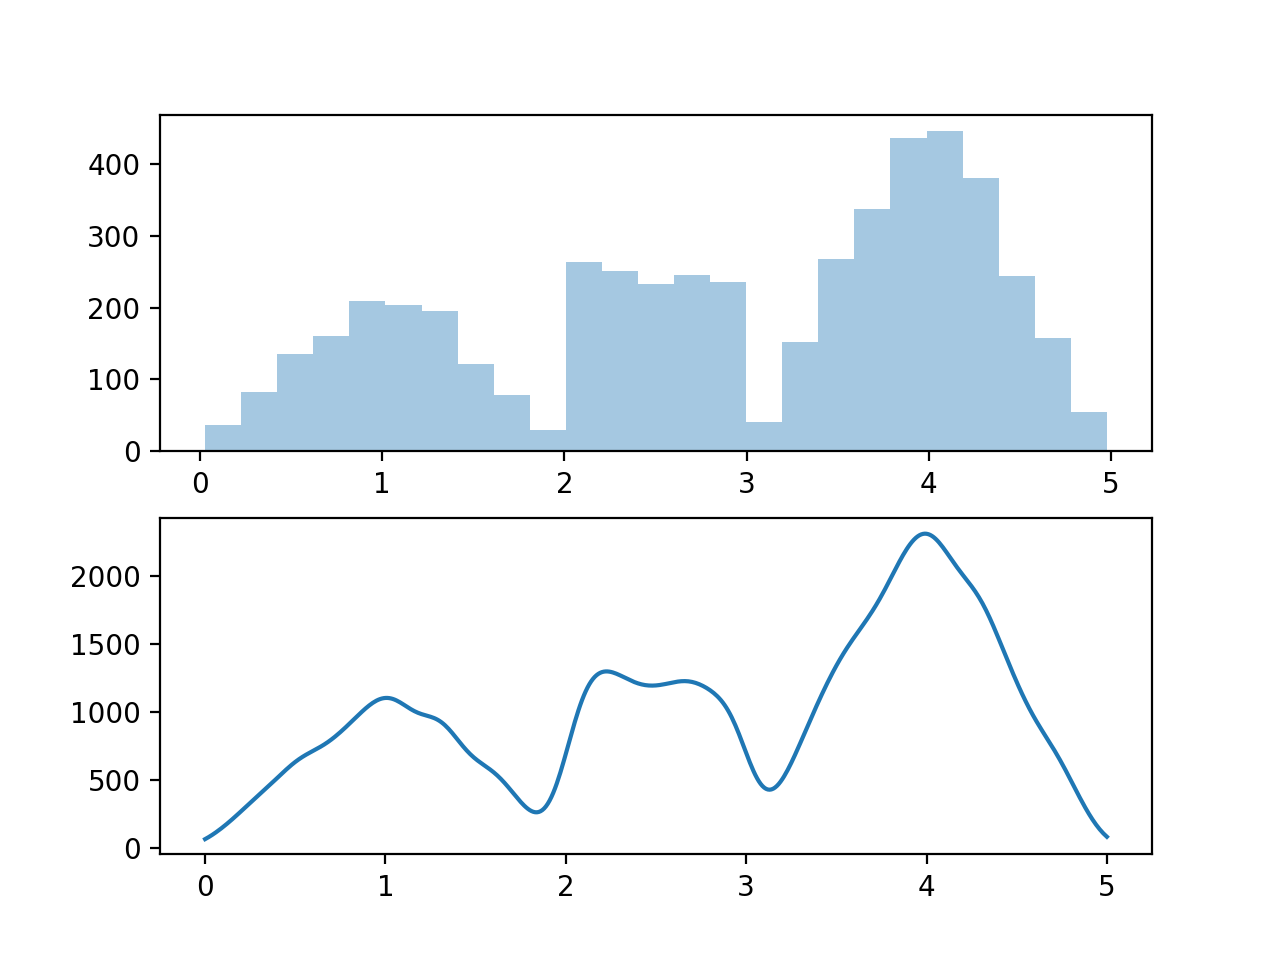
\includegraphics[height=8cm]{image/gauss_kernel.png}
    \caption{\footnotesize シミュレーション実行結果}
\end{figure}

\begin{lstlisting}
import numpy as np
import scipy as sp
from numpy.random import randn, rand
import matplotlib.pyplot as plt
import seaborn as sns
from scipy.stats import norm


def myrand(n=5000):
    x = np.zeros(n)
    u = rand(n)
    flag = (0 <= u) * (u < 1/8)
    x[flag] = np.sqrt(8*u[flag])
    flag = (1/8 <= u) * (u < 1/4)
    x[flag] = 2 - np.sqrt(2 - 8*u[flag])
    flag = (1/4 <= u) * (u < 1/2)
    x[flag] = 1 + 4*u[flag]
    flag = (1/2 <= u) * (u < 3/4)
    x[flag] = 3 + np.sqrt(4*u[flag] - 2)
    flag = (3/4 <= u) * (u <= 1)
    x[flag] = 5 - np.sqrt(4 - 4*u[flag])
    return x


def gkernel_est(sample, x=np.linspace(0, 5, 501), bandwidth=0.1):
    pxh = np.zeros_like(x)
    n = sample.shape[0]
    for i in range(n):
        pxh = pxh + norm.pdf(x, loc=sample[i], scale=bandwidth)
    return x, pxh


def cross_validation(sample, n_split=5, params=[0.01, 0.1, 0.5]):
    n_params = len(params)
    likelihoods = np.zeros(n_params)
    group = np.split(sample, n_split)
    for j in range(n_params):
        for i in range(n_split):
            if i==0:
                sample_temp = np.hstack(group[i+1:][0])
            elif i==n_split-1:
                sample_temp = np.hstack(group[0:i])
            else:
                sample_temp = np.hstack([np.hstack(group[0:i]), group[i+1:][0]])
            _, pxh = gkernel_est(sample_temp, group[i], bandwidth=params[j])
            likelihoods[j] += np.sum(np.log(pxh))
    opt_param = params[np.argmax(likelihoods)]
    #print(likelihoods)
    return opt_param


if __name__ == '__main__':
    np.random.seed(1)
    sample = myrand()
    opt_b = cross_validation(sample=sample)
    x, pxh = gkernel_est(sample=sample, bandwidth=opt_b)

    # plot original samples
    fig = plt.figure()
    ax1 = fig.add_subplot(2,1,1)
    sns.distplot(sample, kde=False, rug=False, bins=25)
    None

    # plot estimated distribution
    ax2 = fig.add_subplot(2,1,2)
    ax2.plot(x, pxh)
    plt.show()

\end{lstlisting}


\newpage
\section*{宿題2: kNN法による文字識別}

kNN法による手書き文字認識を行った.言語はpython.最近傍数$k$は交差確認により決定した.
(正答率の計算部分のみ,scikit-learnのモジュールを用いた.)
訓練データを用いて$k \in \{1,2,3,4,5,10,20\}$について交差確認を行ったところ,$k^* = 1$が最適になった.(交差確認におけるそれぞれの平均正答率は,$[0.9676,  0.9676,  0.9674,  0.9688,  0.965,   0.959,   0.9454]$となった.)
$k:=1$としてテストデータを識別したところ,正答率は,$0.965$となった.


\begin{lstlisting}
import numpy as np
from collections import Counter
from sklearn.metrics import accuracy_score


class kNN(object):
    def __init__(self, k=1):
        self._train_data = None
        self._target_data = None
        self._k = k


    def fit(self, train_data, target_data):
        self._train_data = train_data
        self._target_data = target_data


    def predict(self, x):
        distances = np.array([np.linalg.norm(p - x) for p in self._train_data])
        nearest_indices = distances.argsort()[:self._k]
        nearest_labels = self._target_data[nearest_indices]
        c = Counter(nearest_labels)
        return c.most_common(1)[0][0]


def load_train_data():
    for i in range(10):
        if i==0:
            train_feature = np.loadtxt('data/digit_train{}.csv'.format(i), delimiter=',')
            train_label = np.array([i]*train_feature.shape[0])
        else:
            temp_feature = np.loadtxt('data/digit_train{}.csv'.format(i), delimiter=',')
            train_feature = np.vstack([train_feature, temp_feature])
            temp_label = np.array([i]*temp_feature.shape[0])
            train_label = np.hstack([train_label, temp_label])
            
    return train_feature, train_label


def load_test_data():
    for i in range(10):
        if i==0:
            test_feature = np.loadtxt('data/digit_test{}.csv'.format(i), delimiter=',')
            test_label = np.array([i]*test_feature.shape[0])
        else:
            temp_feature = np.loadtxt('data/digit_test{}.csv'.format(i), delimiter=',')
            test_feature = np.vstack([test_feature, temp_feature])
            temp_label = np.array([i]*temp_feature.shape[0])
            test_label = np.hstack([test_label, temp_label])
            
    return test_feature, test_label


def calc_accuracy(train_feature, train_label, test_feature, test_label, k=1):
    model = kNN(k)
    model.fit(train_feature, train_label)
    predicted_labels = []
    for feature in test_feature:
        predicted_label = model.predict(feature)
        predicted_labels.append(predicted_label)
    return accuracy_score(test_label, predicted_labels)


def load_train_data_cv(n_split=5):
    for i in range(10):
        if i==0:
            train_feature = np.loadtxt('data/digit_train{}.csv'.format(i), delimiter=',')
            train_label = np.array([i]*train_feature.shape[0])
            group_feature = np.split(train_feature, n_split)
            group_label = np.split(train_label, n_split)
        else:
            temp_feature = np.loadtxt('data/digit_train{}.csv'.format(i), delimiter=',')
            temp_group_feature = np.split(temp_feature, n_split)
            temp_label = np.array([i]*temp_feature.shape[0])
            temp_group_label = np.split(temp_label, n_split)
            
            for m in range(n_split):
                group_feature[m] = np.vstack([group_feature[m], temp_group_feature[m]])
                group_label[m] = np.hstack([group_label[m], temp_group_label[m]])
            
    return group_feature, group_label


def cross_validation(n_split=5, params=[1,2,3,4,5,10,20]):
    n_params = len(params)
    score_list = np.zeros(n_params)
    group_feature, group_label = load_train_data_cv(n_split)
    
    for j in range(n_params):
        for i in range(n_split):
            temp_group_feature = group_feature.copy()
            temp_test_feature = temp_group_feature.pop(i)
            temp_train_feature = np.vstack(temp_group_feature)
            
            temp_group_label = group_label.copy()
            temp_test_label = temp_group_label.pop(i)
            temp_train_label = np.hstack(temp_group_label)
            
            score_list[j] += calc_accuracy(temp_train_feature, temp_train_label, temp_test_feature, temp_test_label, k=params[j])/n_split

    opt_param = params[np.argmax(score_list)]
    print(score_list)
    return opt_param


def main():
    k_opt = cross_validation(n_split=5, params=[1,2,3,4,5,10,20])
    train_feature, train_label = load_train_data()
    test_feature, test_label = load_test_data()
    score = calc_accuracy(train_feature, train_label, test_feature, test_label, k=k_opt)
    print(score)


if __name__ == '__main__':
    main()

\end{lstlisting}


\end{document}